
\documentclass[a4paper,openany,12pt]{book}
\input{contenido/Incluir.tex}

% Colocar los argumentos definidos
\faculty{INGENIERÍA ELÉCTRICA, ELECTRÓNICA, INFORMÁTICA Y MECÁNICA}
\school{INGENIERÍA INFORMÁTICA Y DE SISTEMAS}
\title{Plataforma Web para la Optimización de la Gestión del TUPA de la UNSAAC}
\memberOne{Cabeza Huillca Flavio Antony}
\codeOne{211265}
\memberTwo{Mamani Flores Natan}
\codeTwo{230970}
\memberThree{Polo Chura Marco Rosauro}
\codeThree{141632}
\memberFour{Ramos Alata Hernan Washington}
\codeFour{221989}
\memberFive{Vitorino Marin Efrain}
\codeFive{160337}

\docente{Ing. Quispe Sota Julio Vladimir}

%Iniciar el documento
\begin{document}
% Iniciar numeración en romanos
\pagenumbering{roman}
\maketitle % Caratula
\doublespacing
\begin{presentacion}
\vspace{1cm}

\noindent
\textbf{DOCENTE:} \\
Ing. Julio Vladimir Quispe Sota

\vspace{0.3cm}

\noindent
Tenemos el honor de presentar ante usted el proyecto académico titulado:

\vspace{0.4cm}

\begin{center}
    \Large
    \textbf{``Plataforma Web para la Optimización de la Gestión del TUPA de la UNSAAC''}
\end{center}

\vspace{0.8cm}

\noindent
El presente trabajo ha sido desarrollado como parte de las actividades académicas del curso, aplicando conocimientos relacionados con ingeniería de software, desarrollo web, diseño de interfaces modernas y gestión digital de procesos administrativos.

\vspace{0.4cm}

\noindent
El proyecto propone una solución tecnológica orientada a mejorar la administración y automatización de los procedimientos establecidos en el Texto Único de Procedimientos Administrativos (TUPA) de la Universidad Nacional de San Antonio Abad del Cusco, permitiendo optimizar la atención de trámites universitarios mediante una plataforma web moderna, eficiente y accesible.

\vspace{0.4cm}

\noindent
Durante el desarrollo se aplicaron metodologías de análisis, diseño y programación, integrando herramientas y tecnologías actuales para construir un prototipo funcional enfocado en la experiencia del usuario, la transparencia administrativa y la digitalización de procesos institucionales.

\vspace{0.4cm}

\noindent
Esperamos que el presente proyecto cumpla con las expectativas académicas planteadas y contribuya como una propuesta innovadora para la mejora de los servicios administrativos universitarios.

\vspace{1.2cm}

\begin{flushright}
\textbf{Atentamente:} \\[0.4cm]
Los integrantes del equipo:
\end{flushright}

\vspace{0.5cm}

\begin{flushright}
Cabeza Huillca Flavio Antony \\
Mamani Flores Natan \\
Polo Chura Marco Rosauro \\
Ramos Alata Hernan Washington \\
Vitorino Marin Efrain
\end{flushright}

\end{presentacion}

\newpage
\addcontentsline{toc}{chapter}{ÍNDICE}
\tableofcontents

\newpage
\addcontentsline{toc}{chapter}{ÍNDICE DE TABLAS}
\listoftables

\newpage
\addcontentsline{toc}{chapter}{ÍNDICE DE FIGURAS}
\listoffigures

\setlength{\tabcolsep}{10pt}
\clearpage
\pagenumbering{arabic} % Numeracion normal

\newpage
\chapter{ÁMBITO DE APLICACIÓN O INFLUENCIA}

\section{Descripción del ámbito}

\lipsum[1]

\section{Área de influencia}

\lipsum[1]

\section{Beneficiarios}

\lipsum[1]

\newpage
\chapter{DESCRIPCIÓN DE LA PROBLEMÁTICA}

\section{Situación actual}

\lipsum[1-2]

\section{Formulación del problema}
\subsection{Problema general}

\lipsum[1][1-3]

\subsection{Problemas específicos}

\begin{itemize}
    \item Problema específico 1
    \item Problema específico 2
    \item Problema específico 3
    \item Problema específico 4
\end{itemize}

\section{Justificación}

\lipsum[1]

\newpage
\chapter{OBJETIVOS DE LA PROPUESTA}

\section{Objetivo general}

\lipsum[1][1-3]

\section{Objetivos específicos}

\begin{itemize}
    \item Objetivo específico 1
    \item Objetivo específico 2
    \item Objetivo específico 3
    \item Objetivo específico 4
\end{itemize}

\newpage
\chapter{METODOLOGÍA}

% ------------------------------------------------------------
\section{Metodología}
% ------------------------------------------------------------

El presente proyecto adopta \textbf{Scrum} como metodología de desarrollo, un marco de
trabajo ágil ampliamente utilizado en proyectos de software que demandan flexibilidad,
entregas incrementales y colaboración continua entre los integrantes del equipo.

\subsection{Justificación de la elección}

Scrum resulta idóneo para este proyecto por las siguientes razones:

\begin{itemize}
    \item \textbf{Adaptabilidad a cambios:} los requerimientos del TUPA pueden evolucionar
            durante el levantamiento de información con las oficinas de la UNSAAC; Scrum
            permite incorporar estos cambios de forma ordenada en cada sprint.
    \item \textbf{Entregas rápidas e incrementales:} al dividir el desarrollo en sprints de
            duración fija, se obtienen avances funcionales verificables al final de cada
            iteración, facilitando la retroalimentación oportuna del docente y los usuarios.
    \item \textbf{Trabajo colaborativo:} el equipo está conformado por cinco integrantes con
            roles complementarios; Scrum define responsabilidades claras y promueve la
            comunicación constante mediante ceremonias estructuradas.
    \item \textbf{Transparencia y seguimiento:} el uso de tableros de tareas y herramientas
            como Jira permite visualizar el estado del proyecto en todo momento, favoreciendo
            la trazabilidad de actividades y el cumplimiento de los indicadores establecidos
            en el plan de monitoreo.
\end{itemize}

\subsection{Fases del ciclo de desarrollo}

El ciclo de vida del proyecto se estructura en las siguientes fases, ejecutadas de forma
iterativa a lo largo de los sprints planificados:

\begin{enumerate}
    \item \textbf{Planificación:} definición del alcance del sprint, estimación de historias
            de usuario y asignación de tareas al equipo.
    \item \textbf{Análisis:} levantamiento y refinamiento de requerimientos funcionales y no
            funcionales del sistema, en coordinación con las oficinas administrativas de la
            UNSAAC.
    \item \textbf{Diseño:} elaboración de prototipos de interfaz en Figma, diseño de la
            arquitectura del sistema y modelado de la base de datos.
    \item \textbf{Implementación:} desarrollo de los módulos frontend y backend conforme a
            las historias de usuario aprobadas en cada sprint.
    \item \textbf{Pruebas:} verificación funcional, pruebas de integración y validación de
            usabilidad con usuarios representativos.
    \item \textbf{Despliegue:} publicación de incrementos en el entorno de producción y
            monitoreo de disponibilidad y rendimiento del sistema.
\end{enumerate}

\subsection{Herramientas de gestión}

El seguimiento del proyecto se realizará principalmente mediante \textbf{Jira}, herramienta
que permite gestionar el backlog del producto, planificar sprints, registrar el avance de
tareas y controlar los indicadores de desempeño definidos en el plan de monitoreo. De
forma complementaria, se utilizará \textbf{GitHub} para el control de versiones del código
fuente y la gestión de incidencias técnicas.

\subsection{Roles del equipo Scrum}

La siguiente tabla describe los roles Scrum asignados a cada participante del proyecto:

\begin{table}[H]
\centering
\caption{Roles Scrum del equipo de desarrollo}
\label{tab:roles_scrum}
\begin{tabular}{|p{5cm}|p{3.5cm}|p{6cm}|}
\hline
\textbf{Integrante} & \textbf{Rol Scrum} & \textbf{Responsabilidad principal} \\
\hline
Ing. Julio Vladimir Quispe Sota & Product Owner &
Definir y priorizar el backlog del producto; validar que los entregables cumplan con
las necesidades administrativas del TUPA. \\
\hline
Ramos Alata Hernan Washington & Scrum Master &
Facilitar las ceremonias Scrum, eliminar impedimentos y velar por el cumplimiento
del proceso ágil en el equipo. \\
\hline
Vitorino Marin Efrain & Developer – Backend &
Desarrollar la lógica de negocio, API REST y gestión de base de datos; delegar y
coordinar subtareas del módulo backend. \\
\hline
Mamani Flores Natan & Developer – Frontend &
Implementar las interfaces de usuario; delegar y coordinar subtareas del módulo
frontend en coordinación con el diseñador UX/UI. \\
\hline
Cabeza Huillca Flavio Antony & Developer – UX/UI &
Diseñar prototipos en Figma, definir la guía de estilos y coordinar la experiencia
de usuario en toda la plataforma. \\
\hline
Polo Chura Marco Rosauro & QA Tester &
Diseñar y ejecutar casos de prueba, reportar defectos en Jira y verificar el
cumplimiento de los criterios de aceptación por sprint. \\
\hline
\end{tabular}
\end{table}

\subsection{Ceremonias y seguimiento}

El equipo ejecutará las siguientes ceremonias Scrum a lo largo del proyecto:

\begin{itemize}
    \item \textbf{Daily meeting (reunión diaria):} sesión de 15 minutos en la que cada
            integrante comparte lo que realizó el día anterior, lo que hará ese día y los
            impedimentos que enfrenta. Permite detectar bloqueos de forma temprana.
    \item \textbf{Sprint planning (planificación del sprint):} al inicio de cada sprint, el
            equipo selecciona las historias de usuario del backlog, las estima en puntos y las
            descompone en tareas concretas asignadas a cada desarrollador en Jira.
    \item \textbf{Sprint review (revisión del sprint):} al cierre de cada sprint, se
            presenta el incremento funcional al Product Owner y, cuando corresponda, a los
            docentes responsables, para obtener retroalimentación formal.
    \item \textbf{Sprint retrospective (retrospectiva):} el equipo reflexiona sobre el proceso
            de trabajo, identifica áreas de mejora y define acciones concretas para el
            siguiente sprint.
\end{itemize}

% ------------------------------------------------------------
\section{Actividades principales}
% ------------------------------------------------------------

A continuación se describen las actividades principales del proyecto, organizadas conforme
al cronograma establecido. Cada actividad es liderada por un integrante responsable, quien
además delega y coordina las subtareas correspondientes entre los demás miembros del equipo.

\begin{description}

    \item[Actividad 1: Reunión y planificación del proyecto.]
    Consiste en la constitución formal del equipo, la definición del alcance general del
    proyecto, la elaboración del cronograma de actividades y la configuración de las
    herramientas de gestión (Jira, GitHub). Se establecen los acuerdos de comunicación
    interna y se realiza la primera sesión de Sprint Planning. Esta actividad es liderada
    por el \textbf{Scrum Master (Ramos Alata Hernan Washington)}, quien coordina la
    organización del equipo y la asignación inicial de roles y responsabilidades.

    \item[Actividad 2: Levantamiento de requerimientos.]
    Comprende la identificación y documentación de los requerimientos funcionales y no
    funcionales del sistema mediante entrevistas semiestructuradas con las oficinas
    administrativas de la UNSAAC, análisis del TUPA vigente y revisión de documentación
    institucional. Los resultados se registran como historias de usuario en el backlog de
    Jira. Esta actividad es liderada por el \textbf{QA Tester (Polo Chura Marco Rosauro)},
    quien dirige el análisis de requerimientos y delega la elaboración de fichas de
    entrevista y documentos de especificación al resto del equipo.

    \item[Actividad 3: Diseño de prototipos en Figma.]
    Se elaboran los wireframes y prototipos interactivos de alta fidelidad de la plataforma,
    incluyendo la guía de estilos, el sistema de componentes visuales y los flujos de
    navegación para cada tipo de usuario (estudiante, personal administrativo y jefe de
    oficina). Los prototipos son validados con usuarios representativos antes de iniciar el
    desarrollo. Esta actividad es liderada por el \textbf{desarrollador UX/UI (Cabeza
    Huillca Flavio Antony)}, quien diseña los prototipos y coordina los ajustes con el
    equipo frontend.

    \item[Actividad 4: Diseño de la base de datos.]
    Incluye el modelado conceptual, lógico y físico de la base de datos del sistema,
    definiendo entidades, relaciones, restricciones de integridad y procedimientos
    almacenados necesarios para soportar los módulos de gestión de trámites, usuarios y
    reportes. El modelo es revisado y aprobado por el Product Owner antes de su
    implementación. Esta actividad es liderada por el \textbf{desarrollador backend
    (Vitorino Marin Efrain)}, quien diseña el esquema de la base de datos y delega la
    documentación del modelo al equipo.

    \item[Actividad 5: Desarrollo de interfaces gráficas e implementación del módulo
    frontend.]
    Comprende la traducción de los prototipos aprobados en Figma a código, implementando
    las vistas, componentes y flujos de interacción de la plataforma web. Se aplican
    buenas prácticas de desarrollo frontend, diseño responsivo y accesibilidad. Esta
    actividad es liderada por el \textbf{desarrollador frontend (Mamani Flores Natan)},
    quien coordina la implementación de interfaces y delega el desarrollo de componentes
    específicos a los demás integrantes.

    \item[Actividad 6: Integración de módulos e implementación de notificaciones y
    validaciones.]
    Se integran los módulos frontend y backend del sistema, incluyendo el motor de
    notificaciones (correo electrónico y notificaciones en plataforma) y los mecanismos
    de validación documental. Se verifican los contratos de la API REST y la correcta
    comunicación entre componentes. Esta actividad es liderada por el \textbf{desarrollador
    backend (Vitorino Marin Efrain)}, quien coordina la integración técnica y gestiona los
    ajustes necesarios con el equipo frontend.

    \item[Actividad 7: Pruebas y corrección de errores.]
    Abarca la ejecución de pruebas funcionales, de integración y de usabilidad sobre los
    módulos desarrollados. Los defectos identificados se registran en Jira y se priorizan
    para su corrección en el sprint correspondiente. Se verifica el cumplimiento de los
    criterios de aceptación definidos en las historias de usuario. Esta actividad es
    liderada por el \textbf{QA Tester (Polo Chura Marco Rosauro)}, quien diseña los casos
    de prueba y coordina las sesiones de validación con usuarios finales.

    \item[Actividad 8: Elaboración de documentación final y presentación del proyecto.]
    Comprende la redacción de la documentación técnica y académica del proyecto (memoria
    del sistema, manual de usuario, informe final), la preparación de la presentación ante
    los docentes y la entrega formal de todos los artefactos del proyecto. Esta actividad
    es liderada por el \textbf{Scrum Master (Ramos Alata Hernan Washington)}, quien
    coordina la consolidación de la documentación y delega la redacción de secciones
    específicas a cada integrante según su área de responsabilidad.

\end{description}
\newpage
\chapter{INFRAESTRUCTURA Y RECURSOS}

\section{Infraestructura tecnológica}

\lipsum[1]

\section{Recursos humanos}

\lipsum[1]

\section{Recursos materiales}

\lipsum[1]

\newpage
\chapter{EVALUACIÓN Y MONITOREO}

\section{Indicadores de evaluación}

\lipsum[1]

\section{Mecanismos de monitoreo}

\lipsum[1]

\section{Hitos de control}

\lipsum[1]

\newpage
\chapter{RESULTADOS ESPERADOS}

Al concluir el proyecto, se espera que la plataforma web desarrollada genere un impacto
medible tanto en la eficiencia de la gestión administrativa del TUPA como en la experiencia
de los distintos actores de la comunidad universitaria. Los resultados se clasifican en
beneficios cuantitativos y cualitativos, y se alinean directamente con los ocho objetivos

\section{Resultados cuantitativos}
Los siguientes indicadores de resultado proyectan el impacto esperado de la solución una vez
desplegada en producción y adoptada por la comunidad universitaria:

{\small
\begin{tabular}{|p{3.9cm}|c|c|p{2.6cm}|}
\hline
\textbf{Resultado esperado} & \textbf{Línea base (est.)} & \textbf{Meta} & \textbf{OE relacionado} \\
\hline
Reducción del tiempo promedio de atención por trámite & 5–7 días hábiles & $\leq$ 3 días hábiles & OE-03, OE-04 \\
\hline
Reducción de consultas presenciales innecesarias en ventanilla & 100\% presencial & $\leq$ 30\% presencial & OE-01, OE-02 \\
\hline
Incremento en la tasa de trámites resueltos en primer intento & $\sim$40\% & $\geq$ 75\% & OE-03, OE-05 \\
\hline
Porcentaje de módulos con panel de control operativo & 0\% (no existe) & 100\% & OE-06 \\
\hline
Disponibilidad del sistema en producción & N/A & $\geq$ 99\% mensual & OE-08 \\
\hline
Tiempo de respuesta del sistema (p95) & N/A & $\leq$ 2 segundos & OE-01, OE-08 \\
\hline
Generación automática de reportes administrativos & Manual (0 automatiz.) & $\geq$ 5 tipos de reporte & OE-07 \\
\hline
\end{tabular}
}

\textit{Nota: Los valores de línea base son estimaciones obtenidas del análisis de la
problemática descrita. Serán validados con las oficinas administrativas
durante la fase de levantamiento de requerimientos.}

\section{Resultados cualitativos}

\begin{itemize}
    \item \textbf{Mejora de la experiencia de usuario:} La plataforma ofrecerá una interfaz
    moderna, intuitiva y responsiva, reduciendo la curva de aprendizaje para estudiantes y
    personal administrativo sin conocimientos técnicos avanzados (alineado con OE-01).

    \item \textbf{Mayor transparencia institucional:} Los estudiantes podrán consultar en tiempo
    real el estado de sus trámites, los requisitos exigidos y los costos vigentes, eliminando
    la asimetría de información característica del sistema actual (OE-02, OE-04).

    \item \textbf{Centralización y consistencia de la información:} La solución integrará los
    procedimientos de distintas oficinas en un único punto de acceso, evitando duplicidades
    y versiones desactualizadas del TUPA (OE-02, OE-06).

    \item \textbf{Reducción de la sobrecarga administrativa:} La automatización de notificaciones
    y validaciones documentales liberará tiempo del personal de ventanilla para tareas de
    mayor valor agregado (OE-04, OE-05).

    \item \textbf{Cultura de toma de decisiones basada en datos:} La generación de reportes y
    estadísticas de trámites procesados facilitará la identificación de cuellos de botella y
    la mejora continua de los procesos administrativos (OE-07).

    \item \textbf{Sostenibilidad y escalabilidad técnica:} El despliegue en infraestructura en la
    nube y el uso de estándares de desarrollo garantizarán la mantenibilidad y posibilidad de
    extensión futura de la plataforma (OE-08).
\end{itemize}

\section{Impacto esperado}

{\small
\begin{tabular}{|p{2.8cm}|p{5.0cm}|p{4.8cm}|}
\hline
\textbf{Actor} & \textbf{Beneficio directo} & \textbf{Indicador de impacto} \\
\hline
Estudiantes & Acceso 24/7 a información del TUPA, registro en línea de solicitudes y seguimiento del estado de trámites & Reducción de tiempos de espera; disminución de traslados presenciales \\
\hline
Personal administrativo & Validación digital de documentos, panel de gestión por oficina, notificaciones automáticas de acciones pendientes & Menor carga manual; reducción de errores en el proceso \\
\hline
Jefes de oficina & Acceso a reportes estadísticos de trámites, monitoreo del desempeño del área y gestión de usuarios del sistema & Mejor visibilidad para toma de decisiones gerenciales \\
\hline
UNSAAC (institución) & Modernización de la imagen institucional, reducción de costos operativos y cumplimiento de estándares de gobierno digital & Mejora en indicadores de gestión universitaria \\
\hline
\end{tabular}
}

\section{Alineación con los Objetivos Específicos del Proyecto}

La siguiente matriz evidencia la correspondencia directa entre los resultados esperados y los
ocho objetivos específicos del proyecto, garantizando la trazabilidad requerida por el indicador
de desempeño \textbf{AG-C12.01}:

{\small
\begin{tabular}{|p{1.0cm}|p{4.8cm}|p{6.4cm}|}
\hline
\textbf{OE} & \textbf{Objetivo Específico} & \textbf{Resultado / Entregable asociado} \\
\hline
OE-01 & Mejorar la interfaz y experiencia de usuario & Rediseño UX/UI; puntuación de usabilidad $\geq$ 4.0/5.0 \\
\hline
OE-02 & Facilitar la consulta de procedimientos, requisitos y costos & Módulo de búsqueda y consulta pública del TUPA \\
\hline
OE-03 & Optimizar el registro y seguimiento de trámites & Sistema de gestión de solicitudes con trazabilidad por estado \\
\hline
OE-04 & Implementar notificaciones sobre el estado de los procedimientos & Motor de notificaciones (correo electrónico / en plataforma) \\
\hline
OE-05 & Mejorar la gestión y validación de documentos digitales & Módulo de carga, validación y aprobación de documentos \\
\hline
OE-06 & Panel de control para oficinas administrativas & Dashboard por rol con métricas en tiempo real \\
\hline
OE-07 & Generación de reportes y estadísticas & Motor de reportes exportable (PDF / Excel) \\
\hline
OE-08 & Garantizar accesibilidad y disponibilidad & Despliegue en la nube con SLA $\geq$ 99\%; diseño responsivo \\
\hline
\end{tabular}
}



\newpage
\chapter{PARTICIPANTES}

\section{Equipo interno}

\lipsum[1]

\begin{table}[H]
    \centering
    \caption{Equipo interno del proyecto}
    \begin{tabular}{|l|l|l|}
        \hline
        \textbf{Nombre} & \textbf{Rol} & \textbf{Responsabilidades} \\
        \hline
        Integrante 1 & Desarrollador & Descripción de responsabilidades \\
        \hline
        Integrante 2 & Analista & Descripción de responsabilidades \\
        \hline
        Integrante 3 & Diseñador & Descripción de responsabilidades \\
        \hline
    \end{tabular}
\end{table}

\section{Equipo externo}

\lipsum[1]

\begin{table}[H]
    \centering
    \caption{Equipo externo del proyecto}
    \begin{tabular}{|l|l|l|}
        \hline
        \textbf{Entidad/Persona} & \textbf{Rol} & \textbf{Tipo de participación} \\
        \hline
        Entidad 1 & Asesor externo & Descripción de participación \\
        \hline
        Entidad 2 & Patrocinador & Descripción de participación \\
        \hline
    \end{tabular}
\end{table}

\newpage
\chapter{ASPECTOS ADMINISTRATIVOS}

\section{Gestión del proyecto}

La gestión del proyecto se realiza bajo la metodología Scrum, con sprints de duración de 2 semanas. El equipo utiliza las siguientes herramientas:

\begin{itemize}
    \item \textbf{Jira:} Para la gestión del backlog, planificación de sprints y seguimiento de tareas.
    \item \textbf{GitHub:} Control de versiones y repositorio central del código.
    \item \textbf{Discord / WhatsApp:} Comunicación diaria del equipo.
    \item \textbf{Google Drive:} Almacenamiento de documentación compartida.
\end{itemize}

El Scrum Master (Hernán) es el responsable de facilitar las ceremonias Scrum y eliminar bloqueos. El equipo se reúne diariamente a las 8:00 am para el Daily Meeting.

\section{Estructura organizacional}

El proyecto cuenta con la siguiente estructura organizacional:

\begin{table}[H]
    \centering
    \caption{Estructura organizacional del proyecto}
    \begin{tabular}{|p{4cm}|p{3.5cm}|p{6.5cm}|}
        \hline
        \textbf{Rol} & \textbf{Responsable} & \textbf{Funciones} \\
        \hline
        Scrum Master & Ramos Alata Hernan Washington (221989) & Facilitar ceremonias Scrum, gestionar Jira, coordinar entregas. \\
        \hline
        Product Owner & Equipo (rotativo) & Definir prioridades del backlog, validar entregables. \\
        \hline
        Desarrollador Backend & Vitorino Marin Efrain (160337) & Base de datos PostgreSQL, APIs, lógica del servidor. \\
        \hline
        Desarrollador Frontend & Mamani Flores Natan (230970) & Interfaces web, UI/UX, conexión con backend. \\
        \hline
        Tester & Polo Chura Marco Rosauro (141632) & Pruebas funcionales, reporte de bugs. \\
        \hline
        Soporte Documentación & Cabeza Huillca Flavio Antony (211265) & Redacción y revisión de documentación técnica. \\
        \hline
    \end{tabular}
\end{table}

\section{Comunicaciones}

\subsection{Canales de comunicación}

\begin{itemize}
    \item \textbf{Daily Meeting (8:00 am):} Reunión diaria de 15 minutos para sincronizar avances y bloqueos.
    \item \textbf{Sprint Planning (lunes de inicio de sprint):} Planificación de tareas del sprint.
    \item \textbf{Sprint Review (viernes final de sprint):} Demostración de avances a los docentes.
    \item \textbf{Sprint Retrospective (viernes final de sprint):} Mejora continua del proceso.
\end{itemize}

\subsection{Recursos técnicos y despliegue}

\textbf{Estructura del repositorio:}
\begin{verbatim}
tupaunsaac/
|-- backend/
|   |-- .env.example
|   |-- database/
|   |   |-- schema.sql
|   |   |-- migrate.ts
|   |   `-- seed.ts
|   `-- src/
|-- frontend/
|   |-- .env.example
|   `-- src/
|-- docs/
|   `-- Plan_Proyecto.pdf
`-- docker-compose.yml
\end{verbatim}

\textbf{Variables de entorno:}
\begin{verbatim}
# Backend .env
NODEENV=development
BACKENDURL=http://localhost:8080
FRONTENDURL=http://localhost:3000
PORT=8080

DBDIALECT=postgres
DBHOST=localhost
DBPORT=5432
DBUSER=tupa
DBPASS=tupa
DBNAME=tupa

JWTSECRET=cambia-este-secreto
REDISURI=redis://:tupa@127.0.0.1:6379

# Frontend .env
VITEAPIBASEURL=http://localhost:8080
VITEAPPNAME=Portal de Tramite Documentario UNSAAC
\end{verbatim}

\subsection{Configuración y despliegue}

\textbf{Desarrollo local:}
\begin{verbatim}
docker compose up -d postgres redis
cd backend && npm install && npm run dev
cd frontend && npm install && npm run dev
\end{verbatim}

\textbf{Base de datos:}
\begin{verbatim}
cd backend
npm run db:migrate   # Ejecuta schema.sql
npm run db:seed      # Carga datos de prueba
npm run db:setup     # Migrate + Seed
\end{verbatim}

\textbf{Despliegue en producción (Ubuntu 24.x):}
\begin{verbatim}
# Instalar dependencias
sudo apt-get update && sudo apt-get upgrade -y
sudo apt-get install -y build-essential postgresql-client git

# Instalar Node 24.x
curl -fsSL https://deb.nodesource.com/setup_24.x | sudo -E bash -
sudo apt-get install -y nodejs

# Instalar Docker
curl -fsSL https://get.docker.com -o get-docker.sh
sudo sh get-docker.sh
sudo usermod -aG docker ${USER}

# PostgreSQL con Docker
docker volume create tupa_postgres_data
docker run --name tupa-postgres -e POSTGRES_DB=tupa -e POSTGRES_USER=tupa -e POSTGRES_PASSWORD=tupa -p 5432:5432 -d --restart=always -v tupa_postgres_data:/var/lib/postgresql/data postgres:17

# Redis con Docker
docker run --name tupa-redis -p 6379:6379 -d --restart=always redis:latest redis-server --appendonly yes --requirepass "tupa"

# Clonar y desplegar
git clone https://github.com/lovito99/tupaunsaac.git
cd tupaunsaac/backend && npm install && npm run build && npm run db:migrate
cd ../frontend && npm install && npm run build
\end{verbatim}

\subsection{Enlaces útiles}

\begin{itemize}
    \item \textbf{Repositorio GitHub:} \url{https://github.com/Natanmamani/ProyectoDesarrollo}
    \item \textbf{Prototipo Figma:} \url{https://figma.com/...} (Agregar enlace real)
    \item \textbf{Jira:} \url{https://...} (Agregar enlace real)
\end{itemize}

\subsection{Contacto de soporte}

Para consultas relacionadas con el despliegue y soporte técnico, contactar a: \texttt{lovito99\_m@live.com}

\newpage
\chapter{CRONOGRAMA}

\begin{table}[H]
    \centering
    \caption{Cronograma de actividades del proyecto}
    \resizebox{\textwidth}{!}{%
    \begin{tabular}{|p{5cm}|c|c|c|c|c|c|c|c|c|c|c|c|}
        \hline
        \multirow{2}{*}{\textbf{Actividad}} & \multicolumn{12}{c|}{\textbf{Meses - Gestión 2026}} \\
        \cline{2-13}
        & \textbf{Ene} & \textbf{Feb} & \textbf{Mar} & \textbf{Abr} & \textbf{May} & \textbf{Jun}
        & \textbf{Jul} & \textbf{Ago} & \textbf{Sep} & \textbf{Oct} & \textbf{Nov} & \textbf{Dic} \\
        \hline

        Reunión y planificación del proyecto
        & & & & \cellcolor{gray!40} & \cellcolor{gray!40} & & & & & & & \\
        \hline

        Levantamiento de requerimientos
        & & & & & \cellcolor{gray!40} & \cellcolor{gray!40} & & & & & & \\
        \hline

        Análisis de la problemática del TUPA
        & & & & & \cellcolor{gray!40} & \cellcolor{gray!40} & & & & & & \\
        \hline

        Diseño de prototipos en Figma
        & & & & & & \cellcolor{gray!40} & \cellcolor{gray!40} & & & & & \\
        \hline

        Diseño de la base de datos
        & & & & & & \cellcolor{gray!40} & \cellcolor{gray!40} & & & & & \\
        \hline

        Desarrollo de interfaces gráficas (GUI)
        & & & & & & & \cellcolor{gray!40} & \cellcolor{gray!40} & & & & \\
        \hline

        Implementación del módulo frontend
        & & & & & & & \cellcolor{gray!40} & \cellcolor{gray!40} & \cellcolor{gray!40} & & & \\
        \hline

        Integración de módulos del sistema
        & & & & & & & & \cellcolor{gray!40} & \cellcolor{gray!40} & & & \\
        \hline

        Implementación de notificaciones y validaciones
        & & & & & & & & & \cellcolor{gray!40} & \cellcolor{gray!40} & & \\
        \hline

        Pruebas y corrección de errores
        & & & & & & & & & & \cellcolor{gray!40} & \cellcolor{gray!40} & \\
        \hline

        Elaboración de documentación final
        & & & & & & & & & & & \cellcolor{gray!40} & \\
        \hline

        Presentación y entrega del proyecto
        & & & & & & & & & & & \cellcolor{gray!40} & \cellcolor{gray!40} \\
        \hline

    \end{tabular}}
\end{table}

\vspace{0.8cm}

\section*{Coordinación de actividades del equipo}

\begin{center}
\begin{tabular}{|c|p{6cm}|p{5cm}|}
\hline
\textbf{Nro.} & \textbf{Integrante} & \textbf{Responsabilidad Principal} \\
\hline
1 & Ramos Alata Hernan Washington (221989) & Scrum Master: Facilitar ceremonias Scrum, gestionar tablero Jira y coordinar entregas. \\
\hline
2 & Vitorino Marin Efrain (160337) & Desarrollador Backend: Diseñar BD PostgreSQL, crear scripts SQL e implementar APIs. \\
\hline
3 & Mamani Flores Natan (230970) & Desarrollador Frontend + UI/UX: Implementar interfaces web, prototipado en Figma y conectar frontend con backend. \\
\hline
4 & Polo Chura Marco Rosauro (141632) & Tester: Realizar pruebas funcionales, reportar bugs y validar criterios de aceptación. \\
\hline
5 & Cabeza Huillca Flavio Antony (211265) & Soporte UI/UX y Documentación: Apoyar en diseño Figma y colaborar en documentación del proyecto. \\
\hline
\end{tabular}
\end{center}

\newpage
\chapter{PRESUPUESTO}

\section{Presupuesto detallado}

\begin{table}[H]
    \centering
    \caption{Presupuesto del proyecto}
    \begin{tabular}{|l|l|c|c|c|}
        \hline
        \textbf{Categoría} & \textbf{Descripción} & \textbf{Cantidad} & \textbf{Costo unit. (S/.)} & \textbf{Total (S/.)} \\
        \hline
        \multirow{3}{*}{Recursos humanos}
            & Desarrolladores & 5 & 1{,}500.00 & 7{,}500.00 \\
            & Analista de sistemas & 1 & 2{,}000.00 & 2{,}000.00 \\
            & Asesor técnico & 1 & 1{,}200.00 & 1{,}200.00 \\
        \hline
        \multirow{3}{*}{Equipamiento}
            & Computadoras portátiles & 5 & 3{,}500.00 & 17{,}500.00 \\
            & Servidor de desarrollo & 1 & 5{,}000.00 & 5{,}000.00 \\
            & Periféricos & 5 & 300.00 & 1{,}500.00 \\
        \hline
        \multirow{2}{*}{Software y licencias}
            & Licencias de software & 5 & 500.00 & 2{,}500.00 \\
            & Hosting y dominio & 1 & 800.00 & 800.00 \\
        \hline
        \multirow{2}{*}{Materiales}
            & Materiales de oficina & --- & --- & 500.00 \\
            & Impresión y encuadernación & --- & --- & 300.00 \\
        \hline
        \multicolumn{4}{|r|}{\textbf{TOTAL}} & \textbf{38{,}800.00} \\
        \hline
    \end{tabular}
\end{table}

\section{Fuentes de financiamiento}

\lipsum[1]

\newpage
\chapter{PROTOTIPADO}

\section{Prototipado dinámico}

\lipsum[1]

\begin{figure}[H]
    \centering
    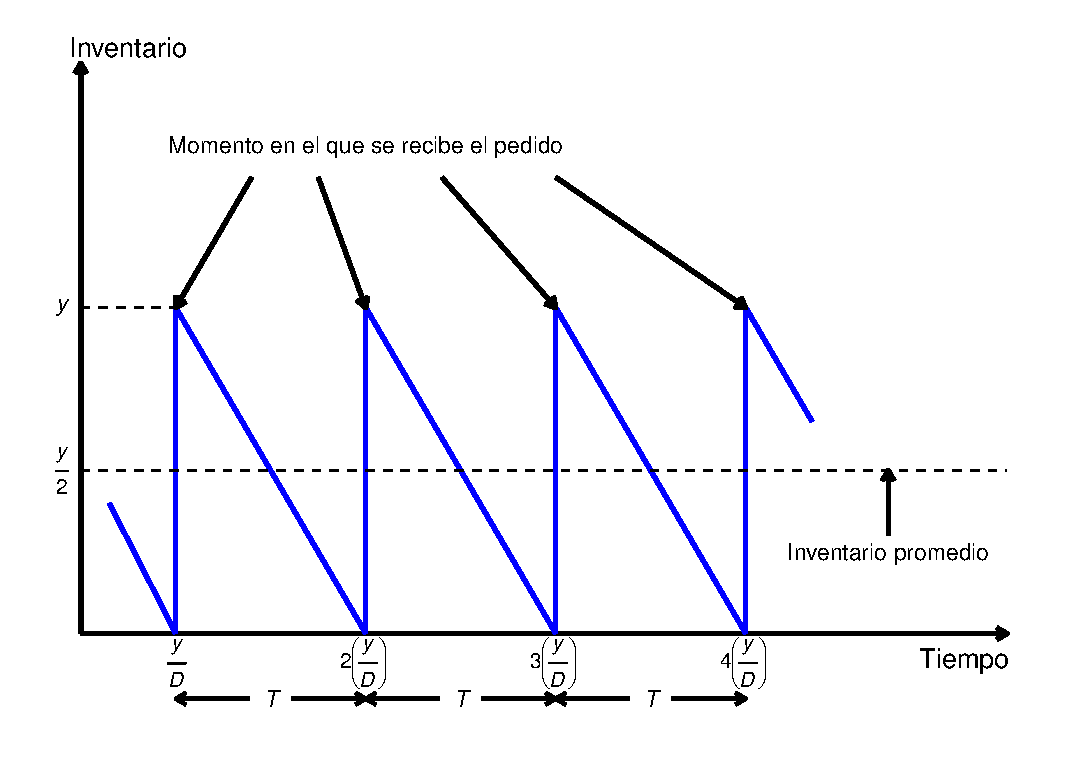
\includegraphics[width=0.85\textwidth]{images/img1}
    \caption{Prototipo dinámico de la interfaz principal}
\end{figure}

\lipsum[1][1-4]


\end{document}
